\documentclass{article}

\usepackage{cite}
\usepackage{fancyhdr}
\usepackage{graphicx}

\pagestyle{fancy}
\lhead{Alex Taylor}
\cfoot{}
\rfoot{\thepage}

\title{Iteration: 4 (16/03 - 22/03)}
\author{Alex Taylor - amt22@aber.ac.uk}

\begin{document}

\maketitle
\begin{center}
	Version 0.4 (Draft)
\end{center}
\tableofcontents
\thispagestyle{empty}
\newpage

\section{Story: Admins can log into the website and run a session with a quiz}
\subsection{Analysis - Breakdown of Tasks}
After doing some spike work last week, this task can now be approached and broken into several sub tasks:
\begin{itemize}
	\item Set up config for Pusher
	\item Add event for broadcasting
	\item Write a command to trigger this event
	\item Add a button to quizzes to trigger this event
	\item Display this on the front end using the javascript which listens for Pusher events
	\item Add a session key box to front page
	\item Add session id to users
	\item Allows admins to change their id
	\item When admin clicks run, this id can be enetered into the key box to join a channel with the name of the id
	\item The user will be presented with the initial quiz page which will be default filled with the name and description of the quiz
	\item The admin will see the same page but with an "admin panel"
	\item This admin panel has a next and previous button for questions
	\item When these buttons are pressed, the question is sent to pusher
	\item These question are rendered as a form on the user end and admin end
	\item The user can submit the form
\end{itemize}
\subsection{Design}
Here are some mockups of the user end of the system (TODO: label and captio these images): 

\begin{center}
	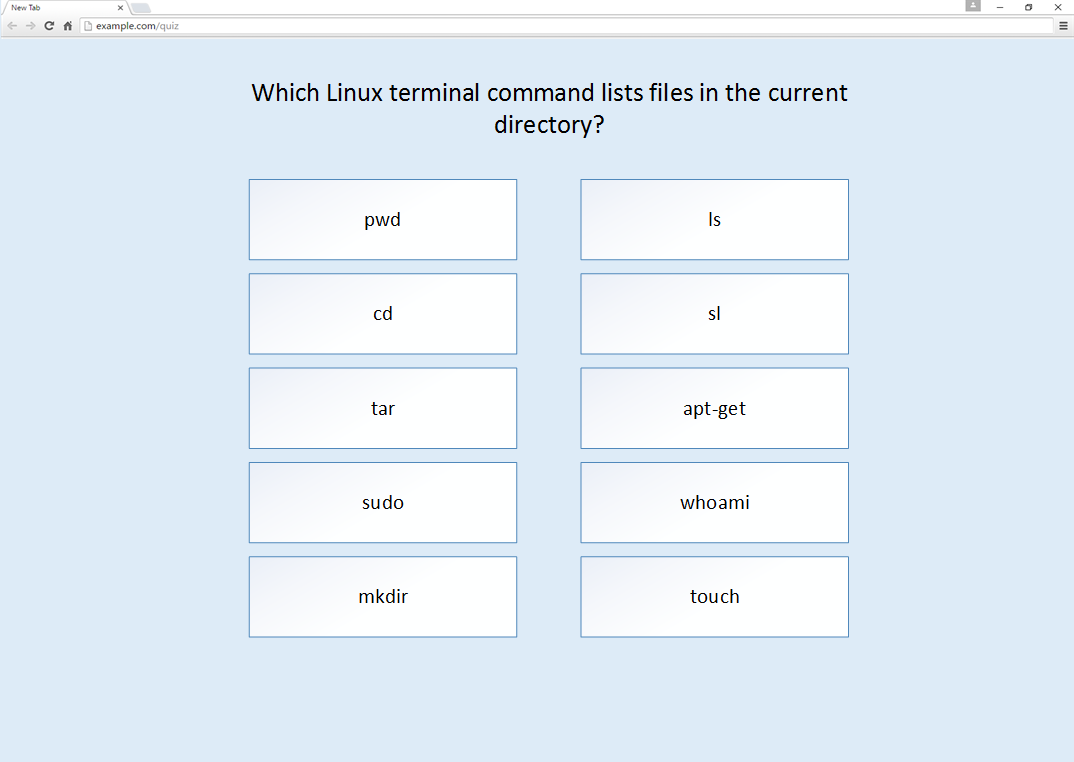
\includegraphics[width=\textwidth]{Quiz-Web-Design-Cropped}\\
	\vspace{1cm}
	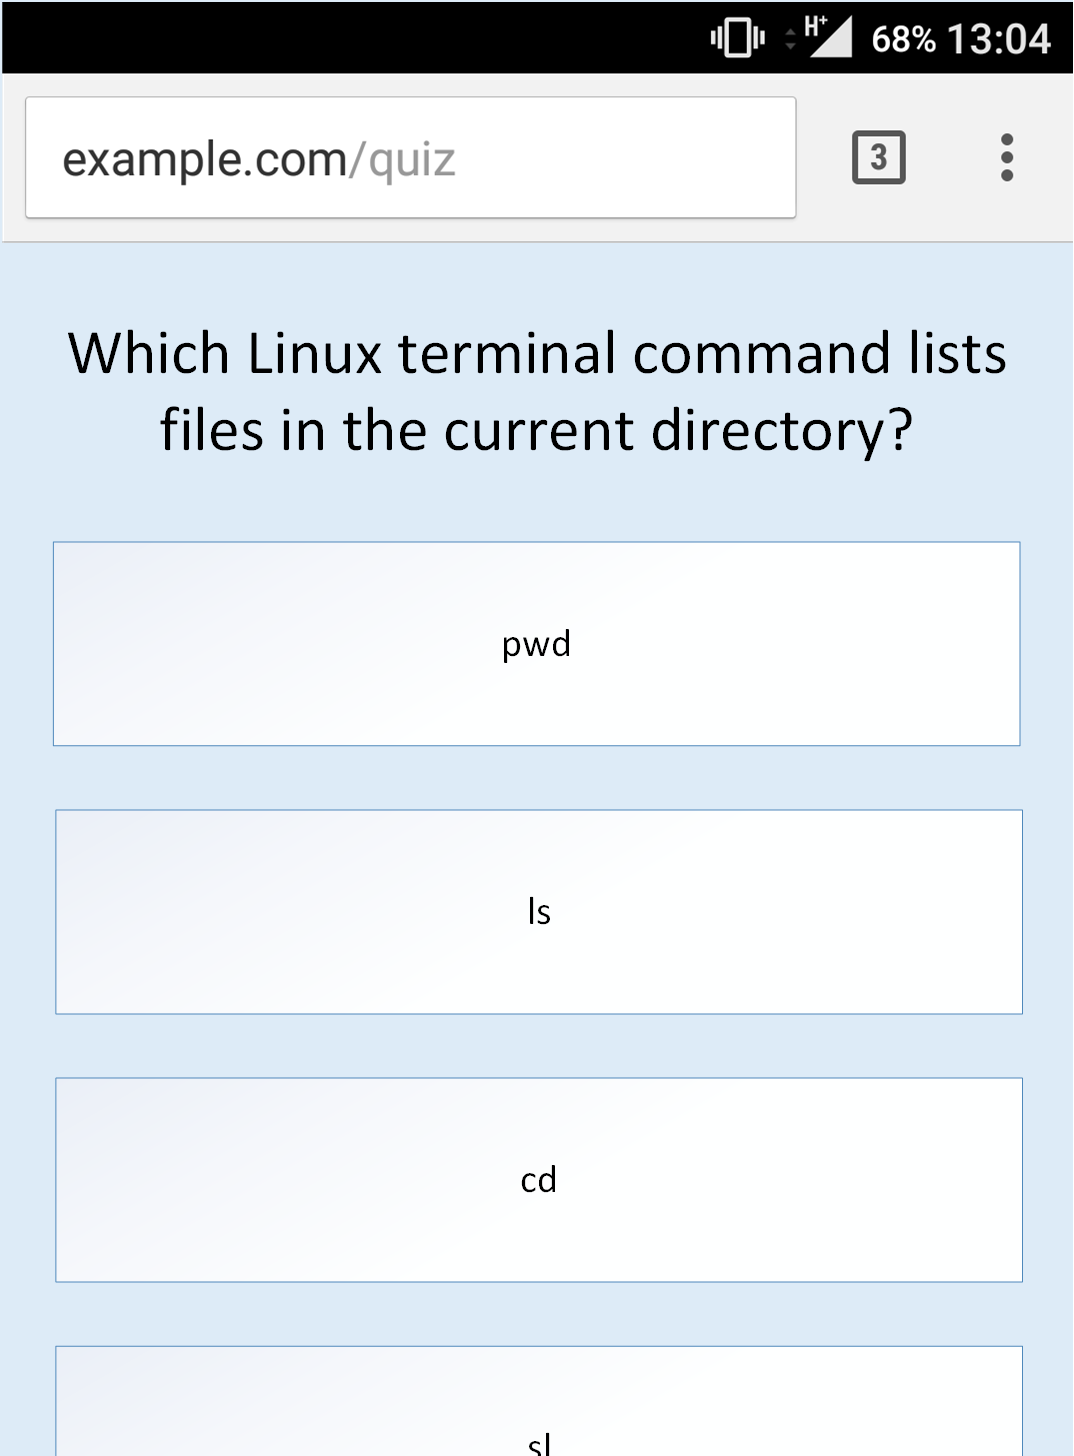
\includegraphics[scale=0.25]{Quiz-Mobile-Cropped}
\end{center}


\subsection{Implementation}
It began by configuring pusher, creating an event and writing some basic javscript to append to the front page. Some work was done on the Admin panel as well, making it only visible to logged in users, and adding the functionality fro previous and next questions. These are just AJAX requests to quiz controller actions which then trigger the event for WebSockets.

Early into the iteration a major flaw with using the WebSockets came up, whilst new content was easy to add to the page, if a new user joined the session late, they would see a blank page/ or the original content of the page that has not yet been removed with javascript. To remedy this, the current position in the quiz should be kept track of and the php on the page should load the question in that position. At the same time, the WebSockets will be running and updating the page from that point onwards in the session. I decided the best place for keeping track was within the session table, which now has appropriate columns for the position, quiz and if it is running.
\subsection{Testing}
No testing as the story is not yet complete.
\newpage

%\section{Bibliography}
%\bibliographystyle{IEEEannotU}
%\bibliography{IEEEabrv,FrameworkHostingBib}

\end{document}